\documentclass{beamer}
\usetheme{CambridgeUS}
\usepackage{graphicx} % Required for inserting images
\usepackage{float}
\usepackage{hyperref}
\usepackage{amsmath}
\usepackage{amsfonts}
\usepackage{amssymb}
\usepackage{dsfont}
\usepackage{adjustbox}
\usepackage{xcolor}
\usepackage{tcolorbox}
\usepackage{multirow}
\usepackage{listings}
\usepackage{xcolor}
\usepackage{minted}
\usepackage[portuguese]{babel}
\usepackage{verbatim}
\usepackage{stackrel}
\usepackage{dsfont}
\usepackage{etoolbox} % Para numeração automática
\usepackage{tcolorbox}
\setbeamertemplate{enumerate items}[default]
\setbeamertemplate{itemize item}{\color{red}$\bullet$}
\setbeamertemplate{enumerate item}{%
  \color{red}%
  \shadowbox{\insertenumlabel}%
}
\setbeamercolor{enumerate item}{fg=gray}
\setbeamercolor{enumerate subitem}{fg=gray}
\setbeamercolor{enumerate subsubitem}{fg=gray}
\setbeamertemplate{enumerate subitem}{\color{gray}(\insertenumlabel)}
\tcbuselibrary{skins, listings} 
% Definindo o contador
\newcounter{exerciciocontador}
\newcounter{definicaocontador}
\newcounter{exemplocontador}
\newcounter{codigocontador}


\definecolor{codegreen}{rgb}{0,0.6,0}
\definecolor{codegray}{rgb}{0.5,0.5,0.5}
\definecolor{codepurple}{rgb}{0.58,0,0.82}
\definecolor{backcolour}{rgb}{1,0.9,0.9}

\lstdefinestyle{mystyle}{
    language=R,
     inputencoding=utf8,
    backgroundcolor=\color{backcolour},   
    commentstyle=\color{codegreen},
    keywordstyle=\color{magenta},
    numberstyle=\tiny\color{codegray},
    stringstyle=\color{codepurple},
    basicstyle=\ttfamily\footnotesize,
    breakatwhitespace=false,         
    breaklines=true,                 
    captionpos=b,                    
    keepspaces=true,                 
    numbers=left,                    
    numbersep=6pt,                  
    showspaces=false,                
    showstringspaces=false,
    showtabs=false,                  
    tabsize=2,
    upquote=true,
     literate=
    {\"}{{\"}}1
    {"}{{"}}1
    {'}{{'}}1
    {“}{{"}}1
    {”}{{"}}1
    {’}{{'}}1
}

\lstset{style=mystyle}


\newtcolorbox{definicao}[1][]{
  enhanced,
  width=\textwidth, % Para ocupar toda a largura disponível
  colback=green!5!white,
  colframe=green!80!black,
  fonttitle=\bfseries\color{black}, % Título em preto
  title={Definição: \quad },
  left=3mm,
  right=3mm,
  top=2mm,
  bottom=2mm,
  sharp corners,
  boxrule=0.9pt,
  drop shadow,
  attach title to upper,
  #1
}

\newtcolorbox{exercicio}[1][]{
  enhanced,
  width=\textwidth, % Para ocupar toda a largura disponível
  colback=blue!5!white,
  colframe=blue!80!black,
  fonttitle=\bfseries\color{black}, % Título em preto
  title={Exercício ~\refstepcounter{exerciciocontador}\theexerciciocontador: \quad },
  left=3mm,
  right=3mm,
  top=2mm,
  bottom=2mm,
  sharp corners,
  boxrule=0.9pt,
  drop shadow,
  attach title to upper,
  #1
}
\newtcolorbox{atencao}[1][]{
  enhanced,
  width=\textwidth, % Para ocupar toda a largura disponível
  colback=red!5!white,
  colframe=red!70!black,
  fonttitle=\bfseries\color{black}, % Título em preto
  title={Atenção: \quad },
  left=3mm,
  right=3mm,
  top=2mm,
  bottom=2mm,
  sharp corners,
  boxrule=0.9pt,
  drop shadow,
  attach title to upper,
  #1
}

\newtcolorbox{exemplo}[1][]{
  enhanced,
  width=\textwidth, % Para ocupar toda a largura disponível
  colback=orange!2!white,
  colframe=orange!40!black,
  fonttitle=\bfseries\color{black}, % Título em preto
  title={Exemplo: \quad },
  left=3mm,
  right=3mm,
  top=2mm,
  bottom=2mm,
  sharp corners,
  boxrule=0.9pt,
  drop shadow,
  attach title to upper,
  #1
}
%\usepackage[hang,small,tight]{subfigure} % subfigura


% \setbeamertemplate{footline}{
%   \hfill%
%   \usebeamercolor[fg]{page number in head/foot}%
%   \usebeamerfont{page number in head/foot}%
%   \setbeamertemplate{page number in head/foot}[framenumber]%
%   \usebeamertemplate*{page number in head/foot}\kern1em\vskip2pt%
% }

%%%%%%%%%%%%%%%% MATHEMATICAL SHORTHANDS %%%%%%%%%%%%%%%%%%%%


\newcommand{\bR}{\mathbb{R}}
\newcommand{\bN}{\mathbb{N}}

\def\P{\mathds{P}}
\def\bE{\mathbb{E}}
\def\mVar{\mbox{Var}}
\def\mDP{\mbox{DP}}
\def\mCov{\mbox{Cov}}
\def\mCor{\mbox{Cor}}
\def\mCV{\mbox{CV}}


\setbeamertemplate{theorems}[numbered]

\AtBeginSection[]{
  \begin{frame}
  \vfill
  \centering
  \begin{beamercolorbox}[sep=8pt,center,shadow=true,rounded=true]{title}
    \usebeamerfont{title}\insertsectionhead\par%
  \end{beamercolorbox}
  \vfill
  \end{frame}
}


\title{Estatística II para Contabilidade - Aulas Práticas}
\author{ Prof. Ismael Bastos}
\date{}

\begin{document}

\begin{frame}
    \titlepage
    \begin{figure}[htpb]
        \begin{center}
            
\includegraphics[width=0.25\linewidth]{figures/arbalest.png}
        \end{center}
    \end{figure}
\end{frame}


\section{Aula 1}
\begin{frame}{Objetivos da aula}
  \begin{itemize}
    \item Entender como funciona a linguagem de programação R.
    \item Como usar o R.
    \item O que é uma variável no contexto do R.
    \item Operações matemáticas no R. 
    \item Como lidar com vetores no R. 
    \item Operações envolvendo vetores. 
    \item Amostragem Aleatória Simples. 
  \end{itemize}
\end{frame}
\begin{frame}{O que é uma linguagem de programação?}
  
  Podemos pensar uma linguagem de programação como sendo uma linguagem do nosso dia-a-dia,
  assim como o português, inglês ou francês. A única diferença é que, no caso das linguagens de programação, 
  o interlocutor é o computador. 

\end{frame}

\begin{frame}{R vs RStudio}
  \begin{figure}
    \begin{center}
            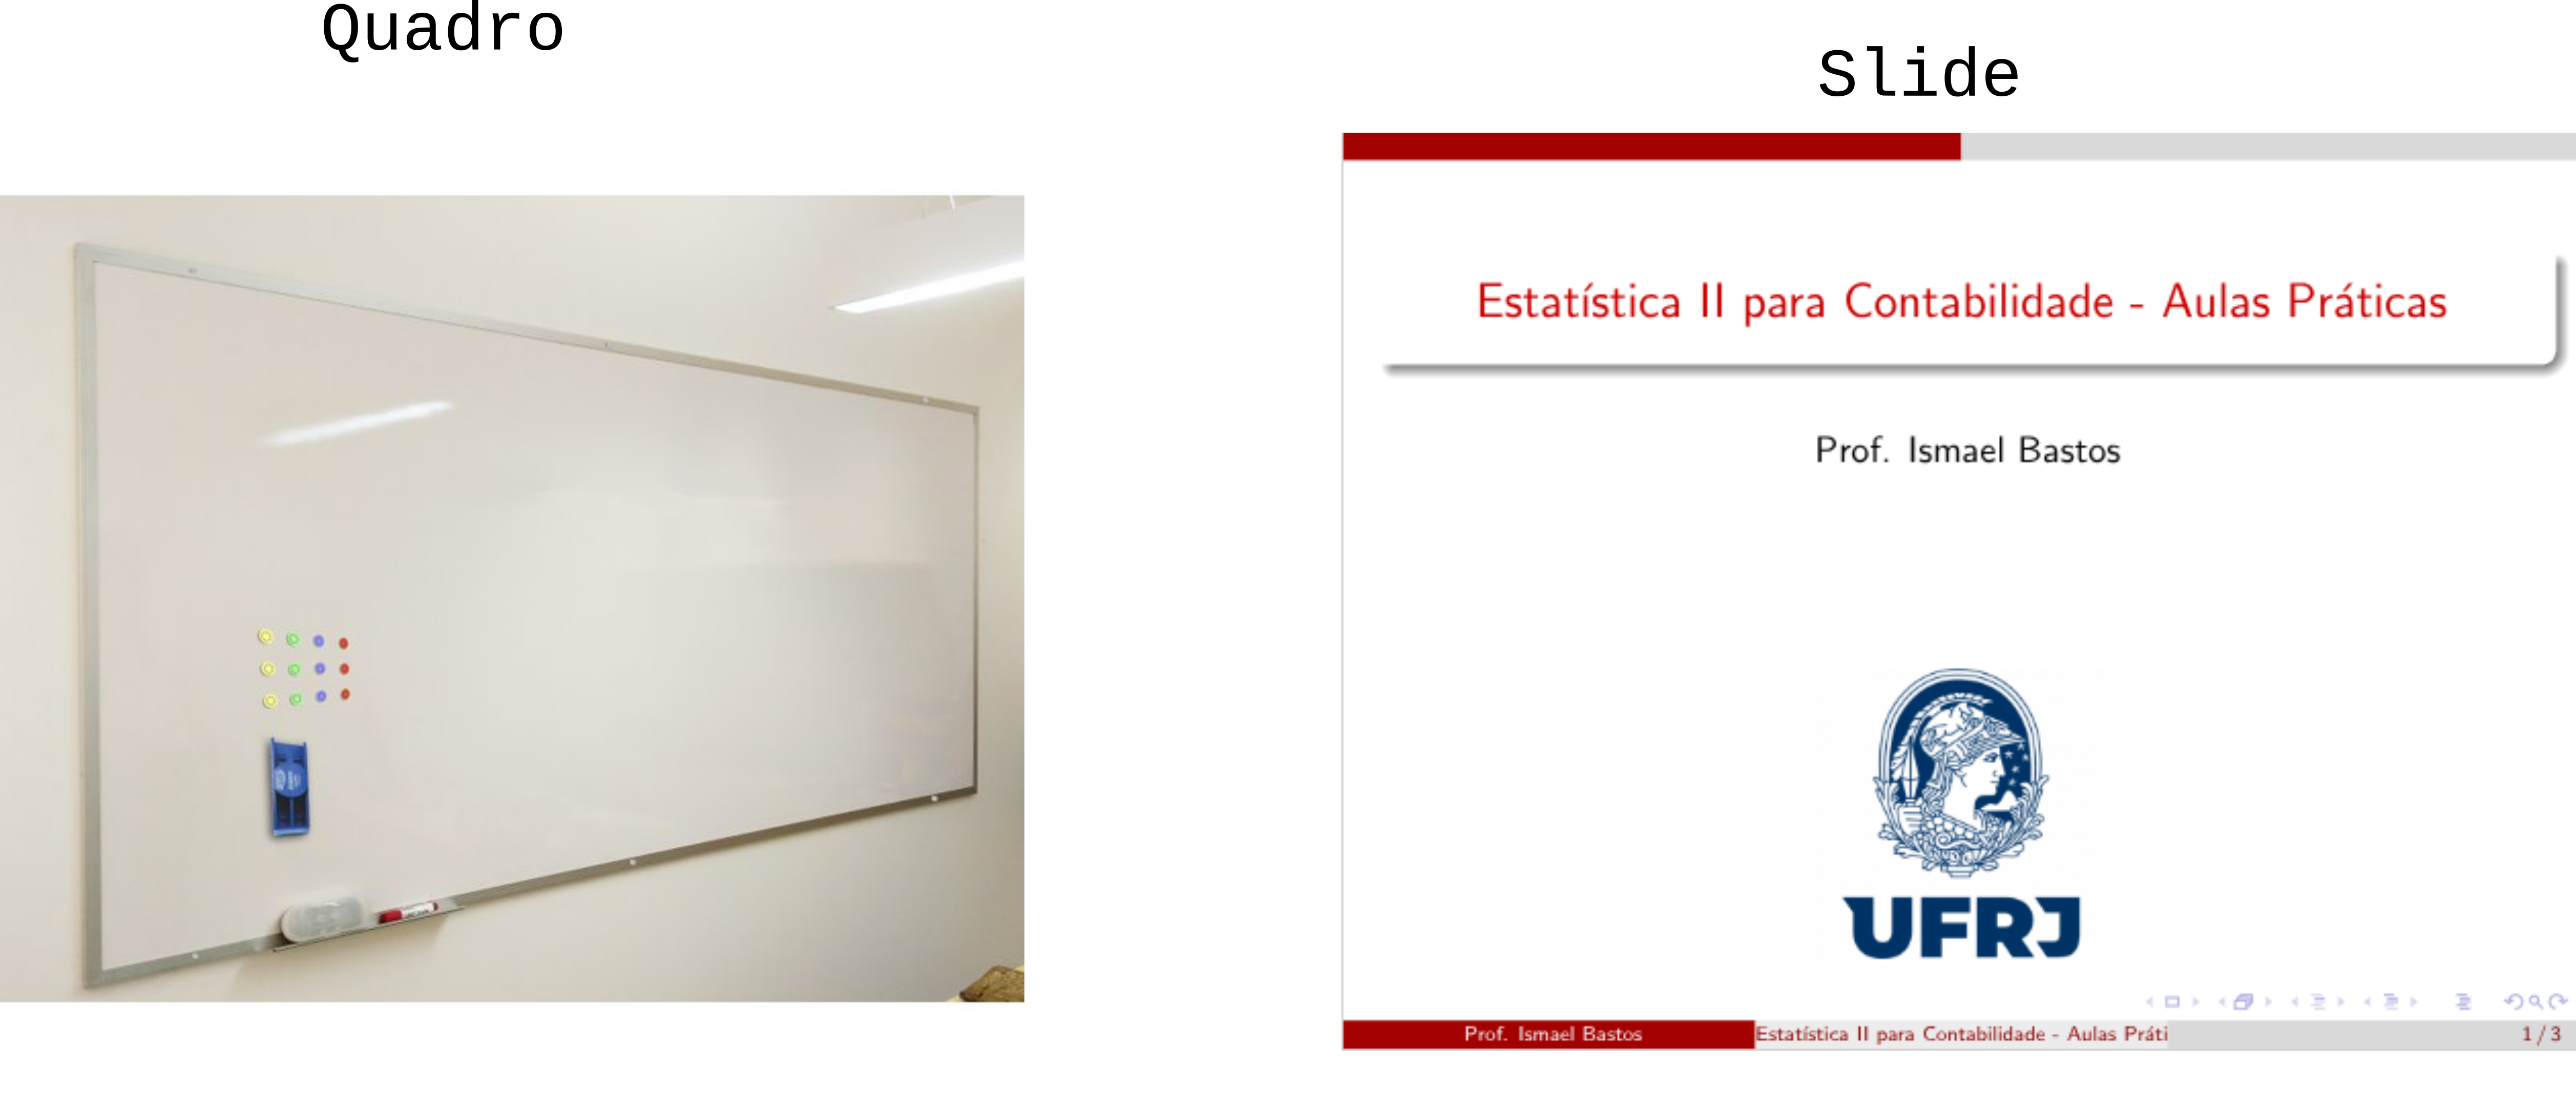
\includegraphics[scale=0.25]{figures/quadro_vs_slide.png}
        \end{center}
  \end{figure}
\end{frame}


\begin{frame}
  \begin{itemize}
    \item Instalando o R
    \item Instalando o RStudio
    \item Usando o Posit Cloud
  \end{itemize}
\end{frame}

\begin{frame}{Variáveis no R}
  \begin{definicao}
  Uma variável no contexto da programação é semelhante ao conceito de variável que vemos em matemática no ensino fundamental.
  Sendo uma incógnita (letra) que guarda um valor. A principal diferença é que ela não assume apenas valores numéricos. 
  \end{definicao}
  
\end{frame}

\begin{frame}{Variáveis no R}
 
  {\color{gray}\large Tipos de variáveis na linguagem R}
 \vspace{0.4cm} % espaço antes do conteúdo
  \begin{itemize}
    \item \textbf{Numérico}(\textit{numeric}): Valores numéricos. Ex: $2, 2.4, 3.14, 42, 616$.
    \item \textbf{Textual}(\textit{character/string}): Valores textuais (Palavras, Frases ou Carácteres). Ex: "André", "Estatística é muito legal", "a", "B", "2", "TRUE"
    \item \textbf{Lógico}(\textit{logical/boolean}): Valores lógicos (Verdadeiro ou Falso). Ex: TRUE, FALSE
  \end{itemize}
\end{frame}

\begin{frame}{Variáveis no R}
\begin{atencao}
\begin{itemize}
  \item Valores numéricos decimais são separados por ponto (.) e não por virgula. 
  \item Valores textuais precisam sempre ser colocados dentro de aspas (Podendo ser aspas duplas ou simples, adote um padrão).
  \item Valores lógicos precisam ser usados com letras em maíusculo, qualquer coisa diferente disso teremos um erro. 
  \item Nomes de variáveis não podem iniciar com caracteres especiais ou números. Ex: 2idade, \_nome, \*casa são nomes não permitidos. 
  \item Nomes de variáveis não podem ser palavras reservadas pela linguagem. Ex: TRUE, FALSE, c, print ...
\end{itemize}
\end{atencao}
\end{frame}

\begin{frame}[fragile]
\frametitle{{Imprimindo valores na tela}}
Para imprimir(mostrar/acessar) os valores armazenados nas variáveis no $R$ podemos simplesmente escrever seu nome e apertar enter. 
Essa forma funciona em praticamente todos os contextos, mas em algums contextos específicos, precisamos usar a função \textit{print}.

\begin{lstlisting}[language=R]
  numero = 5
  print(numero)
\end{lstlisting}
\end{frame}

\begin{frame}{Tarefa 1 - Criando variáveis no R}

  \begin{exercicio}
  Abra o prompt (terminal) do R e faça:

  \begin{enumerate}[a)]
    \item Crie uma variável chamada \textit{nome\_1} e armazene o nome do primeiro membro da dupla.
    \item Crie uma variável chamada \textit{nome\_2} e armazene o nome do segundo membro da dupla.
    \item Imprima na tela os nomes dos membros da dupla. 
    \item Crie uma variável chamada \textit{idade\_1} e armazene a idade do primeiro membro da dupla. 
    \item Crie uma variável chamada \textit{idade\_2} e armazene a idade do segundo membro da dupla.
    \item Imprima na tela as idades dos membros da dupla. 
    \item Imprima na tela a soma das idades dos membros da dupla. 
  \end{enumerate}
  \end{exercicio}
  
\end{frame}

\begin{frame}[fragile]
\frametitle{Operações matemáticas no R} 
  {\color{gray}\large Operações binárias}

  As operações a seguir são operações matemáticas envolvendo dois elementos. No caso do R, esses elementos podem ser números ou variáveis que armazenam valores
  numéricos.
    \begin{itemize}
    \item \textbf{Soma}: Para realizar a soma entre dois elementos no R, utilizamos o símbolo $+$
    \begin{lstlisting}[language=R]
  # Somando números
  s = 10 + 12
  # Somando variaveis
  a = 7
  b = 92
  soma = a + b
  \end{lstlisting}
  \end{itemize}
\end{frame}

\begin{frame}[fragile]
  \frametitle{Operações matemáticas no R} 
  {\color{gray}\large Operações binárias}

  As operações a seguir são operações matemáticas envolvendo dois elementos. No caso do R, esses elementos podem ser números ou variáveis que armazenam valores
  numéricos.
    \begin{itemize}
    \item \textbf{Subtração}: Para realizar a subtração entre dois elementos no R, utilizamos o símbolo $-$
    \begin{lstlisting}[language=R]
  # Subtraindo números
  d = 10 - 12
  # Subtraindo variaveis
  a = 7
  b = 92
  subtr = b - a
  \end{lstlisting}
  \end{itemize}
\end{frame}

\begin{frame}[fragile]
  \frametitle{Operações matemáticas no R} 
  {\color{gray}\large Operações binárias}

  As operações a seguir são operações matemáticas envolvendo dois elementos. No caso do R, esses elementos podem ser números ou variáveis que armazenam valores
  numéricos.
    \begin{itemize}
    \item \textbf{Multiplicação}: Para realizar a multiplicação entre dois elementos no R, utilizamos o símbolo $*$
    \begin{lstlisting}[language=R]
  # Multiplicando números
  m = 10 * 2
  # Multiplicando variaveis
  a = 5
  b = 6
  mult = a * b
  \end{lstlisting}
  \end{itemize}
\end{frame}

\begin{frame}[fragile]
  \frametitle{Operações matemáticas no R} 
  {\color{gray}\large Operações binárias}

  As operações a seguir são operações matemáticas envolvendo dois elementos. No caso do R, esses elementos podem ser números ou variáveis que armazenam valores
  numéricos. 
    \begin{itemize}
    \item \textbf{Divisão}: Para realizar a divisão entre dois elementos no R, utilizamos o símbolo $/$
    \begin{lstlisting}[language=R]
  # Dvidindo números
  m = 10 / 2
  # Dividindo variaveis
  a = 24
  b = 6
  div = a / b
  \end{lstlisting}
  \end{itemize}
\end{frame}


\begin{frame}[fragile]
\frametitle{Operações matemáticas no R} 
  {\color{gray}\large Operações unárias}
As operações a seguir são operações matemáticas envolvendo um elemento. No caso do R, esse elemento pode ser um número ou variável que armazena valores
  numéricos. 
  \begin{itemize}
    \item \textbf{Potência}:Para realizar calcular a $n$-ésima potencia de um elemento usamos o símbolo $^$
    \begin{lstlisting}[language=R]
  # Potenciação de números
  q = 2^2 # dois ao quadrado
  qu =  2^3 # dois ao cubo    
  # Multiplicando variaveis
  a = 5
  b = 4
  mult = a ^ b # cinco elevado a quarta potencia
  \end{lstlisting}
\end{itemize}
\end{frame}


\begin{frame}[fragile]
\frametitle{Operações matemáticas no R} 
  {\color{gray}\large Operações unárias}
As operações a seguir são operações matemáticas envolvendo um elemento. No caso do R, esse elemento pode ser um número ou variável que armazena valores
  numéricos. 
  \begin{itemize}
    \item \textbf{Módulo}:Para calcular o módulo de um elemento usamos a função \textit{abs}.
    \begin{lstlisting}[language=R]
  # Modulo de um número
  n = abs(-2)    # |-2|
  # Modulo de variaveis
  v = -10
  va = abs(v) # |-10|
  \end{lstlisting}
\end{itemize}
\end{frame}

\begin{frame}[fragile]
\frametitle{Operações matemáticas no R} 
  {\color{gray}\large Operações unárias}
As operações a seguir são operações matemáticas envolvendo um elemento. No caso do R, esse elemento pode ser um número ou variável que armazena valores
  numéricos. 
  \begin{itemize}
    \item \textbf{Raiz quadrada}:Para calcular raiz quadrada de um elemento usamos a função \textit{sqrt}.
    \begin{lstlisting}[language=R]
  # Raiz quadrada de números
  q = sqrt(81) # Raiz quadrada de 81 
  # Raiz quadrada de variaveis
  a = 25
  raiz = sqrt(a) # raiz quadrada de 25
  \end{lstlisting}
\end{itemize}
\end{frame}

\begin{frame}{Tarefa 2 - Realizando operações matemáticas no R}
  \begin{exercicio}
    \begin{enumerate}[a)]
      \item Crie duas variáveis chamadas: \textit{v1} e  \textit{v2}.
      \item Obtenha a soma das variáveis.
      \item Obtenha a subtração de $v2$ por $v1$.
      \item Obtenha a divisão entre $v2$ e $v1$.
      \item Obtenha a multiplicação entre as variáveis.
      \item Obtenha a décima potência de \textit{v1}.
      \item Obtenha a raiz quadrada de \textit{v2}.
      \item Obtenha a raiz cúbica de \textit{v2}.
      \item Obtenha  $|-10 \cdot v1|$.
    \end{enumerate}
  \end{exercicio}
\end{frame}

\begin{frame}[fragile]
  \frametitle{Coleção de valores no R - Vetores}

  Podemos também querer armazenar mais de um valor em uma variável. Para fazer isso, 
  usamos a função $c$. 

  \begin{lstlisting}[language=R]
  nomes = c("Jean", "Lucas", "Caio", "Leo")
  idades = c(25, 28, 12, 56)
  print(nomes)
  print(idades)
  \end{lstlisting}
  
  \begin{atencao}
    Todos os valores dentro de um vetor devem ser do mesmo tipo. 
  \end{atencao}
  
\end{frame}

\begin{frame}{Operações envolvendo vetores}
  As mesmas operações que vimos para números funcioina também para vetores desde que ambos 
  possuam apenas elementos do tipo numérico e tenham a mesma quantidade de elementos.
  
  \pause
  \vspace{5px}

  Além disso, podemos realizar operações entre valores numéricos e vetores, o que é equivalente 
  a operação de multiplicação de um vetor por um escalar na matemática. 
  
\end{frame}

\begin{frame}{Acessando elementos de um vetor}

  Cada elemento dentro de um vetor ocupa uma posição específica, sendo essa posição indexada por um número. Nesse caso, 
  a \textcolor{red}{ordem importa}.

Para acessar o elemento que ocupa a posição $i$ de um vetor, basta invocar o vetor passando a posição do elemento entre colchetes. 

\begin{exemplo}
Suponha que tenhamos o seguinte vetor:

$$v = c("A", "U", "L", "A", "1")$$

Para acessar o elemento que ocupa a terceira posição (o valor "L"), devemos escrever $v[3]$
\end{exemplo}
\end{frame}

\begin{frame}{Acessando elementos de um vetor}
 Podemos também acessar múltiplas posições do vetor ao mesmo tempo, basta passar um vetor de posições entre colchetes. 

 \begin{exemplo}
Suponha que tenhamos o seguinte vetor:

$$v = c("A", "U", "L", "A", "1")$$

Para acessar os elementos que ocupam a terceira e quarta posição (o valor "L"), devemos escrever $v[c(3,4)]$
\end{exemplo}

\end{frame}
\begin{frame}{Tarefa 3 - Lidando com vetores no R}

  \begin{exercicio}
    \begin{enumerate}[a)]
      \item Crie um vetor com o nome que você quiser e armazene a idade dos membros de seu grupo e o ano atual.
      \item Crie um vetor com o nome que você quiser e armazene o nome dos membros de seu grupo e o nome da disciplina.
      \item Acesse o elemento que ocupa a segunda posição do vetor do item b).
      \item Acesse os elementos que ocupam a segunda e primeira posição do vetor do item a). 
      \item Multiplique o vetor criado no item a) por 3. 
      \item Calcule a raiz quadrada dos elementos do vetor do item a). 
    \end{enumerate}
  \end{exercicio}
\end{frame}

\begin{frame}[fragile]
    \frametitle{Obtendo o tamanho do vetor}
    Para obter o tamanho de um vetor, utilizamos a função $length$.
  \begin{lstlisting}[language=R]
  nomes = c("Jean", "Lucas", "Caio", "Leo", "Ana", "Vera", "Teo", "Mia", "Ina", "Isa")
  print(length(nomes))
  \end{lstlisting}
\end{frame}

\begin{frame}[fragile]
\frametitle{Amostragem Aleatória Simples}
  Para realizar a Amostragem Aleatória Simples, seguiremos exatamente os passos definidos na aula teórica da disciplina. 

Consideremos o seguinte exemplo de uma população de $10$ pessoas na qual desejamos obter uma amostra de tamanho $3$.
  \begin{lstlisting}[language=R]
  populacao = c("Jean", "Lucas", "Caio", "Leo", "Ana", "Vera", "Teo", "Mia", "Ina", "Isa")
  print(populacao)
  \end{lstlisting}

Vamos atribuir um número a cada um dos elementos da população:
\begin{lstlisting}[language=R]
  populacao = c("Jean", "Lucas", "Caio", "Leo", "Ana", "Vera", "Teo", "Mia", "Ina", "Isa")
  print(populacao)
  populacao_numeros = c(1,2,3,4,5,6,7,8,9,10)
  print(populacao_numeros)
  \end{lstlisting}
\end{frame}

\begin{frame}[fragile]
 \frametitle{Amostragem Aleatória Simples}
 
 Para realizar o sorteio dos números, utiliziaremos a função \textit{sample}. Essa função recebe como argumentos um vetor a ser amostrado e o tamanho da amostra. 
\begin{lstlisting}[language=R]
  populacao = c("Jean", "Lucas", "Caio", "Leo", "Ana", "Vera", "Teo", "Mia", "Ina", "Isa")
  print(populacao)
  populacao_numeros = c(1,2,3,4,5,6,7,8,9,10)
  print(populacao_numeros)
  numeros_amostra = sample(populacao_numeros, 3)
  amostra = populacao[numeros_amostra]
  print(amostra)
  \end{lstlisting}
\end{frame}

\begin{frame}{O que veremos na próxima aula}
  \begin{itemize}
    \item Uso do RStudio.
    \item Amostragem Aleatória Estratificada.
    \item Funções no R. 
    \item DataFrames.
    \item Carregando tabelas Excel no R. 
  \end{itemize}
\end{frame}

\begin{frame}{Exercícios de Fixação (Para Casa)}
  \begin{enumerate}[a)]
    \item Instalar o R ou se ambientar com o Posit Cloud. 
    \item Copie o conjunto de dados presente no arquivo notas.txt e cole no seu prompt (terminal) e o armazene em uma variável.
    \item Considerando esse conjunto de dados como sendo a população de estudo, obtenha uma amostra de tamanho 10. 
    \item Obtenha o sétimo elemento da amostra obtida. 
    \item Obtenha o primeiro, terceiro e quinto elementos da amostra encontrada. 
    \item Refaça os itens a), b) e c). A amostra encontrada é igual a anterior? Por que?
    \item Use o R como calculadora e efetue operações matemáticas e números de sua escolha.
  \end{enumerate}
\end{frame}
\end{document}
